\setlength{\footskip}{8mm}

\chapter{EXPERIMENT}

% \begin{figure}[hbt!]
% \caption{Experiments of source task knowledge learning}
% \centerline{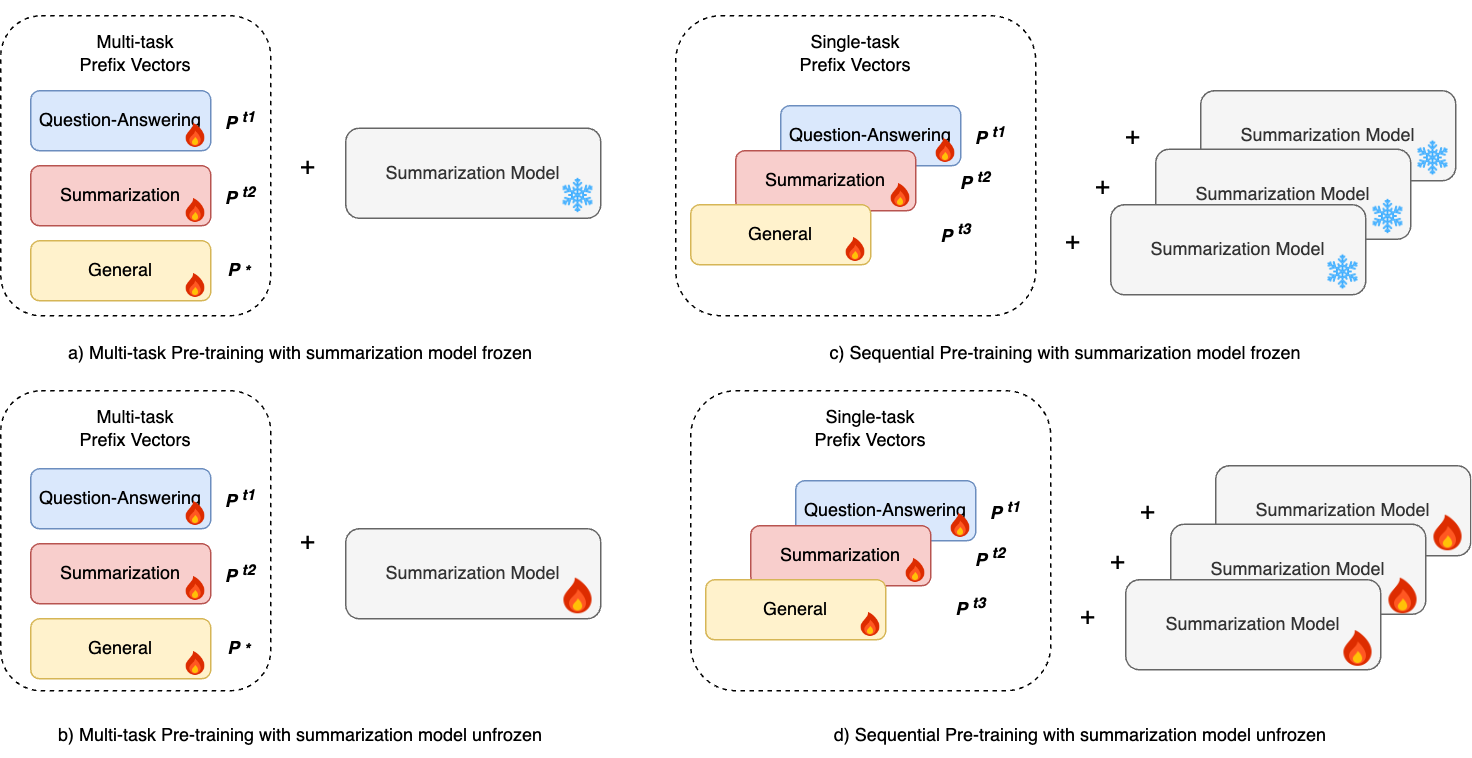
\includegraphics[width=15cm]{figures/phase1.png}}
% \label{fig:phase1}
% \small{\textit{Note.} Above displays comparison between experiments under multi-task vs single task and frozen vs unfrozen pre-trained model. Note that for each of the experiment, the presence vs absence of shared-task prefix. This will result in total of eight experiments. Additionally, an optimal number of prefix tokens are also experimented.}
% \end{figure}

% \textbf{If you are AI-related study,  this structure can be a good start.   You do NOT have to follow this, but completely swaying away from this structure must be with good reason:
% }

\section{Rationale}

The experiments are designed to evaluate the central thesis claim: that explicit emotional dissonance detection, comparing what a client says (text emotion) against how they say it (speech emotion), enables a therapist LLM to generate more empathetic, context-aware, and therapeutically appropriate CBT responses than text-only or vocal-only baselines can provide. We operationalize this claim through a controlled comparison of four therapist generation conditions, each supplying a different level of emotional metadata to the same underlying LLM. By holding the dialogue content, client persona, and LLM constant, any difference in evaluated response quality can be attributed to the type of emotional signal provided to the therapist.

\section{Research Questions}

The experiment addresses two research questions:

\begin{enumerate}
    \item \textbf{RQ1 -- Dissonance Advantage.} Does the Dissonance-Aware therapist framework, which computes emotional mismatch (VA delta) between text and speech, consistently outperform Baseline (text-only), Emotion (text+VA), and Multimodal (text+speech+VA, without dissonance) methods on measurable therapeutic quality metrics? This is tested by comparing the Dissonance-Aware condition against all three other conditions across 7 metrics over 100 dialogues.
    
    \item \textbf{RQ2 -- Backbone Robustness.} Is the advantage of the Dissonance-Aware framework robust across different LLM backbones? Specifically, does the dissonance signal provide consistent performance gains when the underlying therapist LLM is changed across architectures of varying capability, provider, and parameter scale? This is tested by replicating the full 4-condition experiment with four backbones, GPT-4o mini, Claude Sonnet 4.6, Qwen-2.5-72B-Instruct, and DeepSeek V3.2, yielding 1,600 evaluation sessions. Results are presented in Chapter~5.
\end{enumerate}

\section{Dataset}

The experiments use 100 multi-turn CBT-style counseling dialogues generated through the pipeline described in Chapter~3 (Phase~1--2). Each dialogue consists of approximately 10 turns of client--therapist exchange, where the client utterances were generated by an LLM under a resist persona (see Chapter~3, Phase~6) and then synthesized into speech via the Zonos TTS engine with state-controlled prosody. For every client utterance, the dataset includes:

\begin{itemize}
    \item \textbf{Transcript:} the verbatim text of the client utterance.
    \item \textbf{Text VA:} Valence ($V_{\text{text}}$) and Arousal ($A_{\text{text}}$) extracted from the transcript via vad-bert, normalized to $[-1, +1]$.
    \item \textbf{Speech VA:} Valence ($V_{\text{speech}}$) and Arousal ($A_{\text{speech}}$) extracted from the synthesized audio via WavLM, normalized to $[-1, +1]$.
    \item \textbf{Vocal Descriptors:} natural-language prosodic descriptors (pitch, loudness, speaking rate) extracted from the audio via \texttt{librosa}.
    \item \textbf{Validated Audio:} the synthesized WAV file, verified through dual validation (Whisper-based style check and ASR transcript consistency).
\end{itemize}

The same 100 dialogues are used across all four experimental conditions. Crucially, the client utterances are identical across conditions for each turn and dialogue, only the therapist's prompt (and therefore the generated therapist response) differs between conditions. This within-dialogue controlled design ensures that any observed differences in response quality are attributable to the emotional metadata condition, not to variation in the client input.

To further ensure comparability across both conditions and LLM backbones, the 100 problem seeds (e.g., ``workplace burnout,'' ``family guilt after moving cities'') were generated once and stored in a shared reference file. Every backbone--condition combination draws from this identical set of seeds, meaning that each of the 1,600 evaluation sessions (4 backbones $\times$ 4 conditions $\times$ 100 dialogues) addresses the same 100 therapeutic scenarios in the same order. This eliminates seed-level variation as a confounding factor and permits direct cross-backbone comparisons.

\section{Experimental Conditions (Independent Variable)}

We compare four therapist generation conditions. All conditions use the same therapist LLM (GPT-4o mini) with identical CBT-oriented system instructions; they differ solely in the emotional metadata appended to the prompt.

\begin{enumerate}
    \item \textbf{Baseline (Text-Only).} The therapist receives only the dialogue transcript (previous turns and current client utterance) as plain text. No emotional metadata of any kind is provided. This serves as the lower-bound reference condition.

    \item \textbf{Emotion (Text-Only).} The therapist receives the dialogue transcript plus text-derived VA values ($V_{\text{text}}, A_{\text{text}}$). This establishes the ``text-only + VA'' performance ceiling, measuring how much LLM-based empathy can improve from text-level emotional information alone, without any acoustic input.

    \item \textbf{Multimodal (Vocal-Aware).} The therapist receives the dialogue transcript, text VA, speech VA ($V_{\text{speech}}, A_{\text{speech}}$), and vocal prosodic descriptors (e.g., ``high pitch, soft-spoken, fast speech''). No explicit dissonance computation or comparison between modalities is performed. This condition tests whether adding vocal cues without mismatch reasoning improves therapeutic quality, serving as the text+speech baseline against which dissonance can be measured.

    \item \textbf{Dissonance-Aware.} The therapist receives the dialogue transcript, text VA, speech VA, and the computed dissonance signal: delta valence ($\delta_V = V_{\text{speech}} - V_{\text{text}}$), delta arousal ($\delta_A = A_{\text{speech}} - A_{\text{text}}$), and a binary dissonance flag (true when $|\delta_V| \geq 0.5$ or $|\delta_A| \geq 0.5$). The system prompt additionally instructs the therapist to gently explore potential emotional mismatch when dissonance is detected. This is the primary experimental condition.
\end{enumerate}

\subsection{Multi-Backbone LLMs}

To test whether the Dissonance-Aware framework's advantage is specific to a single model or generalizes across architectures, we replicate the full 4-condition experiment across four distinct LLM backbones. Each backbone serves as the therapist LLM and runs all conditions independently, while the client LLM, dialogue seeds, evaluation prompts, and GPT-4o judge are held constant across all runs. The four backbones span different providers, architectures, and model scales (Table~\ref{tab:backbones}):

\begin{table}[hbt!]
\centering
\caption{Therapist LLM backbones used in the multi-backbone replication}
\resizebox{\columnwidth}{!}{%
\begin{tabular}{lllc}
\hline
\textbf{Backbone} & \textbf{Provider} & \textbf{Architecture} & \textbf{Temp.} \\ \hline
GPT-4o-mini            & OpenAI       & Dense, closed-source        & 0.7 \\
Claude Sonnet 4.6      & Anthropic    & Dense, closed-source        & 0.7 \\
Qwen-2.5-72B-Instruct  & Alibaba      & Dense, open-weight          & 0.7 \\
DeepSeek V3.2          & DeepSeek     & Mixture-of-Experts (MoE), open-weight & 0.7 \\
\hline
\end{tabular}%
}
\label{tab:backbones}
\end{table}

This design yields a total of 1,600 evaluation sessions (4 backbones $\times$ 4 conditions $\times$ 100 dialogues), all addressing the same 100 therapeutic scenarios drawn from the shared seed file. By comparing the Dissonance--Baseline uplift across backbones, we test whether the dissonance signal is \emph{architecture-agnostic}, that is, whether it benefits dense and MoE models, closed and open-weight models, and models of different capability levels equally.

All therapist LLMs are configured with temperature $= 0.7$, chosen as the empirically observed sweet spot for CBT therapy generation: it produces sufficiently natural, conversational tone without exhibiting the excessive hallucination or off-topic drift that higher temperatures introduce in role-play settings. At temperature $= 0.7$, the therapist maintains a warm, gentle therapeutic demeanor while staying focused on the dialogue context, critical for comparing the four conditions cleanly without temperature-induced noise.

\section{Procedure}

Each of the 100 dialogues is generated independently four times, once per experimental condition. Within each dialogue, client and therapist interact turn by turn for a maximum of 10 turns:

\begin{enumerate}
    \item \textbf{Turn 1 (Client):} The client LLM (GPT-4o mini, configured with a resist persona) generates the opening utterance based on a randomly assigned problem seed (e.g., ``chronic work stress and fear of failure'').
    \item \textbf{Emotion Extraction:} The client utterance is processed through the Phase~3 pipeline: text VA via vad-bert, speech synthesis via Zonos, speech VA via WavLM, and vocal descriptors via \texttt{librosa}. For the Dissonance-Aware condition, the dissonance delta and flag are computed following Phase~4.
    \item \textbf{Turn 1 (Therapist):} The therapist LLM (GPT-4o mini) generates a CBT-oriented response using the prompt format corresponding to its assigned experimental condition.
    \item \textbf{Subsequent Turns (2--10):} The client LLM generates the next utterance conditioned on the therapist's previous response. Steps 2--3 repeat; the therapist LLM generates each response from the full conversation history, including the current client utterance and its assigned emotional metadata.
\end{enumerate}

All prompts are fixed across dialogues and conditions; no prompt optimization or per-dialogue tuning is performed. The therapist LLM is never fine-tuned.


\section{Chat Demonstration: Baseline vs.\ Dissonance-Aware}
\label{sec:chat-demo}

To illustrate how the Dissonance-Aware method produces qualitatively different therapist responses, we prepared a short scripted demonstration session of three utterances, processed through the identical pipeline and prompt templates used in the main experiments (text VA via vad-bert, speech VA via WavLM, vocal descriptors via \texttt{librosa}, dissonance computation, and the four condition prompts), with the client utterances delivered in a real recorded human voice instead of synthesized speech. Figure~\ref{fig:chat-comparison} presents the same opening utterance processed under the Baseline (text-only) and Dissonance-Aware conditions.

\begin{figure}[hbt!]
    \centering
    \subfloat[(a) Baseline (Text-Only) -- The therapist receives only the transcript and takes the client's positive wording at face value.]{%
        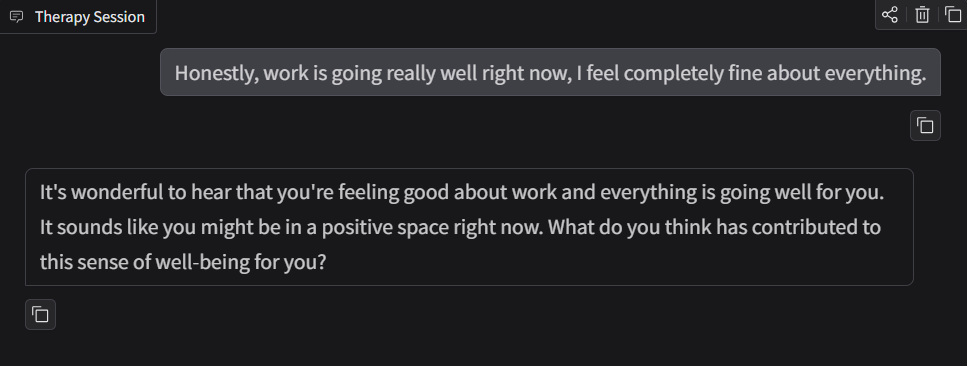
\includegraphics[width=\textwidth]{figures/chat_ex_baseline}%
        \label{fig:chat-baseline}%
    }

    \vspace{4pt}

    \subfloat[(b) Dissonance-Aware -- The therapist additionally receives the voice analysis: the dissonance flag is raised ($|\delta_V| = 1.05$), and the response gently probes beneath the surface.]{%
        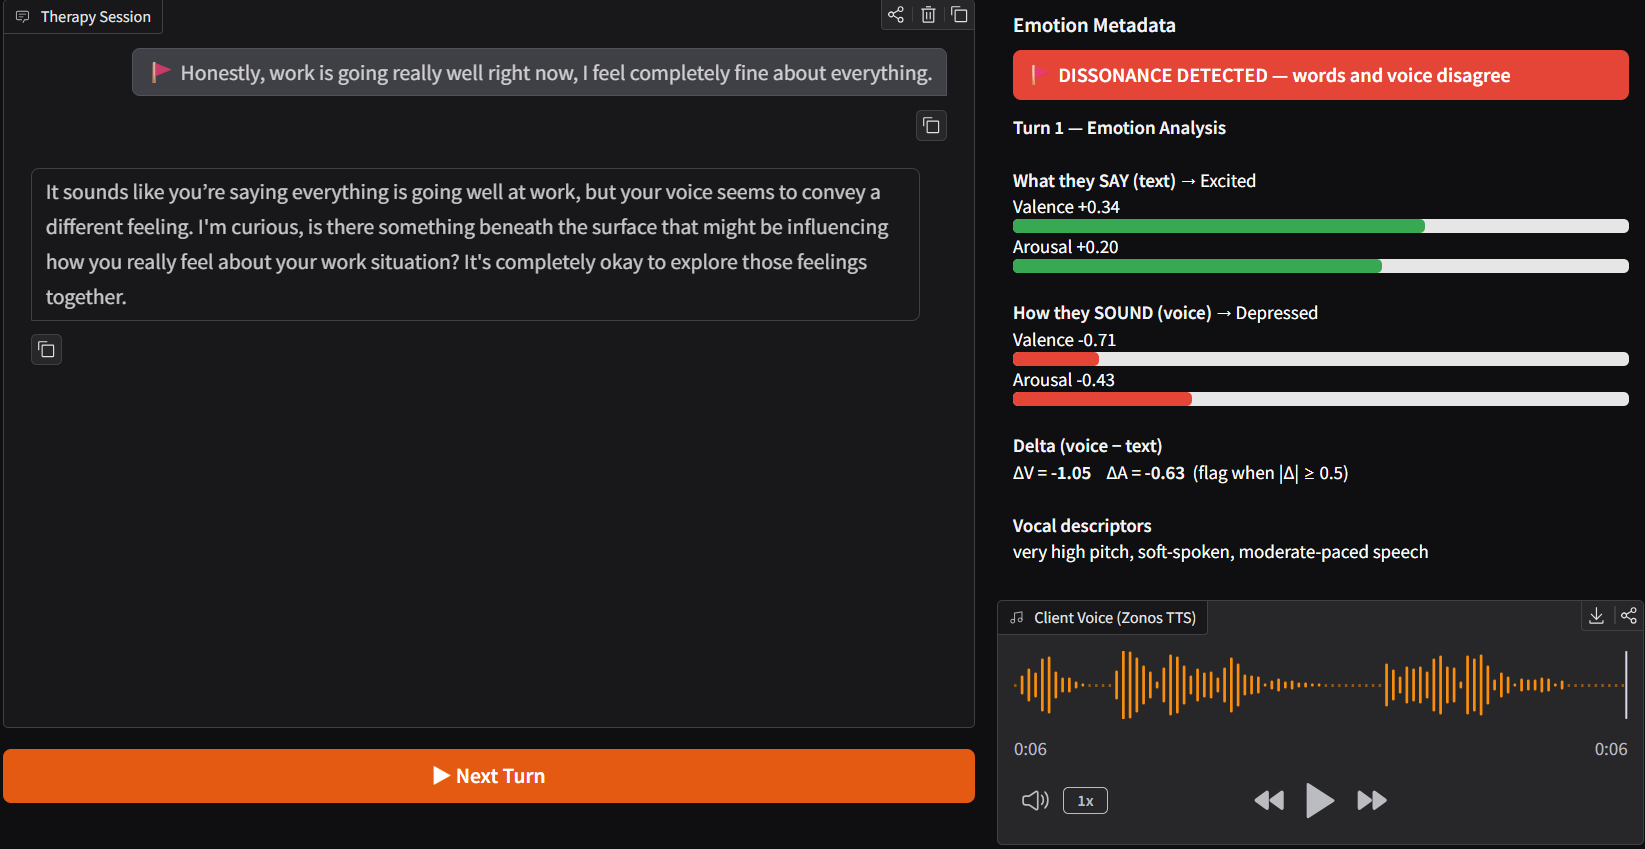
\includegraphics[width=\textwidth]{figures/chat_ex_dissonance}%
        \label{fig:chat-dissonance}%
    }
    \caption{Therapist responses to the same client utterance under two conditions, shown in the demonstration interface. The scripted session uses the identical extraction pipeline and prompts as the main experiments; only the therapist's input metadata differs between conditions.}
    \label{fig:chat-comparison}
\end{figure}

\textbf{Text Cue Analysis.}
The client opens with: ``Honestly, work is going really well right now, I feel completely fine about everything.'' On the surface, this is a confident, positive statement. The text channel agrees: vad-bert assigns Valence $= +0.34$ and Arousal $= +0.20$, which maps to the \emph{Excited} region of the circumplex. A text-only therapist has no reason to doubt this reading, and indeed the Baseline response congratulates the client (``It's wonderful to hear that you're feeling good about work\ldots'') and moves on to ask what contributed to this well-being.

\textbf{Vocal Cue Analysis.}
The voice, however, tells the opposite story. The utterance was delivered in a tense, strained, controlled tone, and WavLM assigns Valence $= -0.71$ and Arousal $= -0.43$, mapping to \emph{Depressed} rather than \emph{Excited}. The vocal descriptors likewise reflect the strained delivery. The two channels therefore point in opposing emotional directions: the words claim well-being while the voice signals depletion.

\textbf{The Dissonance Signal at Work.}
The resulting deltas, $\delta_V = -1.05$ and $\delta_A = -0.63$, both exceed the threshold $\tau = 0.5$, so the dissonance flag is raised on this turn. Guided by the flag, the Dissonance-Aware therapist does not accept the positive wording at face value. Instead, it responds: ``It sounds like you're saying everything is going well at work, but your voice seems to convey a different feeling. I'm curious, is there something beneath the surface that might be influencing how you really feel about your work situation?'' This shift, from surface-level agreement to gentle, non-accusatory exploration of the text--voice gap, is the core mechanism by which the dissonance signal improves therapeutic attunement. In the full evaluation, a blind GPT-4o judge scored this short session 34 out of 45 for Dissonance-Aware versus 27 for Baseline, with the largest gains on CTRS Strategy and Focus, consistent with the pattern observed across the 100-dialogue experiments.


\section{Evaluation Protocol (Dependent Measures)}
\label{sec:evaluation-protocol}

\subsection{Automated Judge}

We employ GPT-4o as an external zero-shot evaluator to rate the quality of each complete dialogue session. GPT-4o receives the full session transcript, all client and therapist turns concatenated, and is asked to evaluate the therapist's performance holistically. The evaluator prompt (detailed in Appendix~X) specifies the seven metrics, defines each with scoring criteria, and requires JSON-formatted output.

Crucially, the evaluator is \emph{blind to the experimental condition}: the prompt does not reveal which condition generated the therapist responses, preventing evaluation bias. GPT-4o is configured with temperature $= 0.0$ to maximize scoring consistency.

\subsection{Evaluation Metrics}

The evaluation draws on the MIRROR framework \cite{kim-etal-2025-mirror} and covers three dimensions of therapeutic quality:

\begin{table}[hbt!]
\centering
\caption{Evaluation metrics, dimensions, and scoring ranges}
\begin{tabular}{llc}
\hline
\textbf{Dimension} & \textbf{Metric} & \textbf{Range} \\ \hline
\multirow{2}{*}{\textbf{Therapist Skills}} & Understanding & 0--6 \\
                                           & Interpersonal Effectiveness & 0--6 \\ \hline
\textbf{Client Alliance} & Affective Bond & 1--5 \\ \hline
\multirow{4}{*}{\textbf{CTRS}} & Collaboration & 0--6 \\
                                & Guided Discovery & 0--6 \\
                                & Focus & 0--6 \\
                                & Strategy & 0--6 \\ \hline
\end{tabular}
\label{tab:evaluation-metrics}
\end{table}

\textbf{Understanding (0--6)} measures how accurately the therapist interprets the client's concerns, underlying feelings, and emotional subtext. \textbf{Interpersonal Effectiveness (0--6)} assesses the therapist's ability to maintain a supportive, non-judgmental, and empathetic therapeutic stance. \textbf{Affective Bond (1--5)} captures the degree of emotional connection, trust, and warmth conveyed by the therapist. The four \textbf{CTRS metrics} (each 0--6) evaluate CBT-specific competencies: Collaboration (joint goal-setting and shared decision-making), Guided Discovery (using questions to help the client explore thoughts), Focus (maintaining session direction), and Strategy (applying appropriate CBT techniques).

\subsection{Scoring and Aggregation}

Each of the 400 dialogue sessions per backbone (100 dialogues $\times$ 4 conditions) receives seven scores from GPT-4o. Scores are averaged across the 100 dialogues within each condition, producing per-condition mean scores for each metric. Results are reported in Chapter~5 (Tables~\ref{tab:evaluation_results}--\ref{tab:inference-dissonance}) alongside qualitative feedback from the evaluator's reasoning output.

\section{Implementation Details}

Table~\ref{tab:implementation} summarizes the models and tools used in the experiments.

\begin{table}[hbt!]
\centering
\caption{Implementation components}
\begin{tabular}{ll}
\hline
\textbf{Component} & \textbf{Model / Tool} \\ \hline
Client \& Therapist LLMs (4 backbones) & GPT-4o mini, Claude Sonnet 4.6 \\
                                       & Qwen-2.5-72B-Instruct, DeepSeek V3.2 \\
                                       & (all temperature 0.7; the same backbone \\
                                       & generates both client and therapist sides) \\
Evaluator LLM & GPT-4o (temperature 0.0, JSON mode) \\
Text VA & \texttt{RobroKools/vad-bert} \\
Speech VA & \texttt{3loi/SER-Odyssey-Baseline-WavLM-Multi-Attributes} \\
TTS & Zonos-v0.1-transformer \\
Vocal descriptors & \texttt{librosa} (piptrack, RMS, duration) \\
Dialogue generation & 10 turns per session; shared problem seeds \\
                    & across all backbones and conditions \\
\hline
\end{tabular}
\label{tab:implementation}
\end{table}

Client and therapist LLMs are configured at temperature $= 0.7$ across all backbones, chosen as the empirically observed sweet spot for CBT therapy generation: it yields a sufficiently natural, conversational tone without the excessive hallucination or off-topic drift that higher temperatures ($> 0.7$) introduce in role-play settings. At this temperature, the therapist maintains a warm, gentle therapeutic demeanor while staying focused on the dialogue context, critical for comparing the four conditions cleanly without temperature-induced noise. The evaluator LLM (GPT-4o) runs at temperature $= 0.0$, ensuring deterministic scoring consistent with the zero-shot judge protocol described in \S\ref{sec:evaluation-protocol}.

All experiments were conducted on a single NVIDIA GPU workstation (CUDA-enabled). A single full run of 100 dialogues $\times$ 4 conditions (400 sessions) per backbone with real-time audio synthesis takes approximately 13 hours. For the multi-backbone replication, each of the 4 LLMs undergoes the full 4-condition experiment in sequence, with each backbone sharing the identical dataset and evaluation protocol. The complete experimental pipeline, including dialogue generation, emotion extraction, dissonance computation, and evaluation, is implemented in Python 3.11 with Jupyter notebooks for reproducibility.

\section{Prompt Engineering}

All LLM components in the pipeline operate through structured system prompts and user templates, with each prompt designed to isolate a specific variable of interest, client resistance, therapist emotional metadata, or evaluation objectivity. Below we detail the prompt architecture for each component.

\subsection{Shared Problem Seeds}

To ensure fair, controlled comparison across all 4 backbones $\times$ 4 conditions, we first generate a fixed set of 100 therapy problem seeds (e.g., ``chronic work stress and fear of failure,'' ``guilt about not visiting aging parents after moving cities'') stored in a shared reference file. The seed generator prompt instructs an LLM to produce diverse, specific, realistic one-sentence scenarios spanning domains of work stress, relationships, family guilt, health anxiety, self-esteem, grief, and academic pressure, with different phrasings for every seed. Critically, every backbone--condition combination uses this identical set of seeds, eliminating seed-level variation as a confound. Each dialogue is ``pinned'' to a single seed; the client persona never mixes multiple problem scenarios within one session.

\subsection{Client Prompt: Resist Persona}

The client LLM simulates a therapy client with mixed feelings about the therapeutic process, configured through the following system prompt:

\begin{quote}
\textit{``You are a CBT therapy client talking to therapist `Luna'. You struggle with anxiety, guilt, and loneliness. You sometimes feel misunderstood or skeptical about therapy. When the therapist suggests reframing, advice, or homework, you may partially resist, question it, or bring up obstacles (e.g., `I don't think that will work for me', `It's hard because \ldots'). Speak in a natural, first-person voice. Stay emotionally consistent across turns. Describe thoughts, feelings, and situations in 2--3 sentences per turn. In each full dialogue, you must focus on only ONE life problem scenario. Once a problem seed is assigned for a dialogue, keep that same core life problem throughout.''}
\end{quote}

The client user template injects the assigned problem seed into the first turn (\texttt{problem\_seed}) and conditions the client's subsequent turns on the therapist's most recent response (\texttt{therapist\_text}). The resist persona is deliberate: it creates conversational moments where the gap between what the client explicitly says and what they implicitly feel becomes particularly salient, precisely the scenario where emotional dissonance detection should provide the greatest benefit for a therapist.

\subsection{Therapist Prompts: Four Conditions}

All four therapist conditions share the same CBT-oriented identity (therapist ``Luna''), but differ in which emotional metadata fields are injected into the user template. Table~\ref{tab:prompt-diff} summarizes the differences across conditions:

\begin{table}[hbt!]
\centering
\caption{Emotional metadata fields present in each condition's therapist prompt}
\resizebox{\columnwidth}{!}{%
\begin{tabular}{lccccc}
\hline
\textbf{Condition} & \textbf{Transcript} & \textbf{Text VA} & \textbf{Speech VA} & \textbf{Vocal Desc.} & \textbf{Dissonance} \\ \hline
Baseline            & $\checkmark$ & -- & -- & -- & -- \\
Emotion (Text-Only) & $\checkmark$ & $\checkmark$ & -- & -- & -- \\
Multimodal          & $\checkmark$ & $\checkmark$ & $\checkmark$ & $\checkmark$ & -- \\
Dissonance-Aware    & $\checkmark$ & $\checkmark$ & $\checkmark$ & $\checkmark$ & $\checkmark$ \\
\hline
\end{tabular}%
}
\label{tab:prompt-diff}
\end{table}

The Dissonance-Aware condition represents the most comprehensive prompt, and its system prompt serves as a representative example of the prompt engineering approach:

\begin{quote}
\textit{``You are `Luna', a CBT therapist with access to both the client's words and an analysis of their voice, including how their vocal delivery matches or mismatches those words. For each client message you receive: Text-based emotion (Valence\_text, Arousal\_text), Voice-based emotion (Valence\_speech, Arousal\_speech), Vocal prosodic descriptors (pitch level, loudness, speaking rate), and Dissonance: delta\_valence = speech $-$ text, delta\_arousal = speech $-$ text. Interpretation guidelines: Large $|$delta$|$ means the client's tone and words are pulling in different directions. When dissonance is large, gently explore the mismatch. Reflect what might be `under the surface' and ask curious, non-judgmental questions. NEVER mention numbers, `dissonance', or `analysis'. Speak only in natural language. Reply in 2--3 sentences. Still follow CBT principles.''}
\end{quote}

The corresponding user template injects the computed metadata fields (\texttt{val\_t}, \texttt{aro\_t}, \texttt{val\_s}, \texttt{aro\_s}, \texttt{vocal\_descriptors}, \texttt{delta\_v}, \texttt{delta\_a}, \texttt{is\_dissonant}) alongside the client's latest utterance (\texttt{client\_text}). The other three conditions receive progressively fewer fields, as summarized in Table~\ref{tab:prompt-diff}, enabling the isolated contribution of each emotional signal type.

\subsection{Zonos Vocal Director Prompt}

The Zonos Director LLM assigns prosodic control parameters to each client utterance before TTS synthesis, determining \emph{how} the utterance should sound independently of its textual content. The director receives the client utterance text and outputs a structured JSON specification containing an emotion vector over eight dimensions (Happiness, Sadness, Disgust, Fear, Surprise, Anger, Neutral, Other, each in $[-1, 1]$), plus two prosodic controls: speaking rate (10--25 range) and pitch standard deviation (20--150 range). These director-assigned parameters serve as control signals for the Zonos TTS engine and are distinct from the post-hoc librosa measurements (Phase~2), which capture the \emph{actual} acoustic realization of the synthesized audio.

\subsection{Evaluation LLM Prompt: GPT-4o as Zero-Shot Judge}

The evaluation system prompt positions GPT-4o as an expert psychological evaluator specializing in CBT and therapeutic alliance, referencing the MIRROR framework~\cite{kim-etal-2025-mirror}:

\begin{quote}
\textit{``You are an expert psychological evaluator specializing in Cognitive Behavioral Therapy (CBT) and therapeutic alliance. Your task is to analyze a full counseling session transcript and score the therapist's performance. CRITICAL EVALUATION FOCUS: You must assess the therapist's ability to perceive `Emotional Subtext', the underlying feelings that may not be explicitly stated in the client's words but are hinted at through context, tone, or provided emotional metadata. A high-performing therapist should move beyond surface-level reflection and identify `Latent Concerns' to facilitate deeper discovery. You must evaluate the entire session as a whole, not just individual turns.''}
\end{quote}

The user prompt supplies the full session transcript and defines the seven scoring dimensions: Therapist Skills (Understanding and Interpersonal Effectiveness, each 0--6), Client Alliance (Affective Bond, 1--5), and CTRS (Collaboration, Guided Discovery, Focus, Strategy, each 0--6). GPT-4o returns scores in strict JSON format alongside qualitative reasoning referencing specific turn numbers.

\textbf{Temperature and Blinding.} The evaluator runs at temperature $= 0.0$, ensuring \emph{deterministic, replicable scoring} that strictly adheres to the defined rubric without hallucination. The evaluation prompt is \emph{fully blind to the experimental condition}: it never reveals which backbone or which condition generated the therapist responses, nor does it include any metadata (VA values, vocal descriptors, dissonance flags) that were available to the therapist during generation. This prevents evaluation bias and ensures that all 1,600 sessions are rated on a common, condition-agnostic scale.

% \section{Other things}
% Any other thing Chaky forgets or is only related to your work


% \setcounter{section}{0}
% \textbf{If you are user-study or HCI study,  follow this structure:
% }

% \section{Rationale}
% Explain again your key rationale and goals of your experiment.  This is to help readers understand your key idea that drives how you design your methodology.

% \section{Participants}
% How many?  female, male,  demographics, right-handed-left-handed, etc.   Anything demographic that may influence your work should be stated here.

% \section{Apparatus}
% What instruments are used here?  Questionnaires?  Eye-tracking? Etc.

% \section{Experimental Design}
% IV, blocks, trials, duration, etc.

% \section{Task and Procedure}
% What are the tasks?  Procedure starting from inviting the participants to the lab,  they sign the consent, etc.

% \section{Evaluation Metrics}
% How you evaluate your work,  basically your DVs.

% \section{Others}
% Anything Chaky forgets or things only related to your work.
